\documentclass[10pt,twocolumn]{article}

\usepackage[margin=0.75in]{geometry}
\usepackage{amsmath,amssymb}
\usepackage{booktabs}
\usepackage{graphicx}
\usepackage{hyperref}
\usepackage{natbib}
\usepackage{enumitem}
\usepackage{caption}

\setlength{\parskip}{0.3em}
\setlength{\parindent}{0em}
\setlength{\bibsep}{0.2em}

\title{\textbf{Social Interaction as Regularization\\for Hierarchical Reinforcement Learning}\\[0.3em]
\large ML8103 Sequential Decision Making --- Final Report}

\author{Vladislav Smirnov \qquad Mirat Aubakirov\\[0.3em]
\textit{Mohamed bin Zayed University of Artificial Intelligence}}

\date{April 2026}

\begin{document}
\maketitle

\section{Introduction}

In hierarchical RL, a manager network picks subgoals and a worker network executes low-level actions~\citep{nachum2018hiro, vezhnevets2017feudal, bacon2017option}. The common failure case is \textbf{goal collapse}: the manager learns to output the same goal every time, which makes the hierarchy useless.

We try two things to fix this. First, we route goals through a \textbf{discrete bottleneck} (Gumbel-Softmax) that forces the manager to pick from a finite set of 1000 messages instead of outputting a continuous vector. Second, we add a \textbf{second agent} that reads the same messages, hoping that the need to coordinate would push goals toward something meaningful.

The second idea did not work the way we expected. The discrete bottleneck alone already prevents collapse almost perfectly. Adding a partner actually reduces goal diversity slightly --- agents develop efficient codes rather than diverse ones.

\section{Method}

\subsection{Environment}

We built a custom 11$\times$11 MiniGrid corridor environment (Figure~\ref{fig:arch}a). Two rooms are connected by a 3-cell-wide passage. The agent starts top-left and has to reach the bottom-right room. Observations are partial (7$\times$7 view). The agent gets $-0.01$ per step and $+1.0$ for reaching the goal. In the two-agent version, agents start in opposite rooms and each has to cross to the other side. They get a $+0.5$ bonus if both finish. Max episode length is 500 steps.

We picked this environment because the corridor creates a natural bottleneck where agents have to pass each other, which is where coordination should matter. The downside (which we only discovered after running experiments) is that flat PPO solves it trivially --- 99.3\% success from the start. More on this in Section~\ref{sec:discussion}.

\subsection{Conditions}

Table~\ref{tab:conditions} lists the six setups we compared. The first wave of experiments (March, 1M timesteps, no-stress corridor) covered the four core HRL conditions; the second wave (April, 100k timesteps, \emph{stress} corridor) added two coordination-aware baselines, LOLA and MADDPG, and re-ran all six modes under a harder configuration designed to keep flat PPO from trivially solving the task.

\begin{table}[h]
\centering
\small
\caption{The six conditions. GS = Gumbel-Softmax. CTDE = centralised training, decentralised execution.}
\label{tab:conditions}
\begin{tabular}{@{}lllc@{}}
\toprule
Condition & Manager & Goals & Agents \\
\midrule
Flat PPO        & ---     & ---                                & 1 \\
HRL Continuous  & TD3     & $\mathbf{g} \in [-1,1]^{16}$       & 1 \\
HRL Discrete    & PPO+GS  & $\mathbf{m} \in \{1,...,10\}^3$    & 1 \\
HRL Social      & PPO+GS  & $\mathbf{m} \in \{1,...,10\}^3$    & 2 \\
HRL+LOLA        & PPO+GS  & $\mathbf{m} \in \{1,...,10\}^3$    & 2 \\
MADDPG          & ---     & continuous action (CTDE)           & 2 \\
\bottomrule
\end{tabular}
\end{table}

To make the comparison between discrete and social fair, we created a single-agent version of the same corridor layout. Both conditions see the same grid, same observations, same rewards. The only difference is whether a second agent is present.

\paragraph{Stress configuration.} The April runs use a harder variant of the corridor: extended episode horizon, an additional wall configuration, and (in two-agent modes) a \emph{bus} sub-task that forces both agents to traverse the same narrow cell within a small time window. This configuration was chosen because the original corridor was solved by flat PPO from the first epoch, leaving no head-room to compare HRL conditions on task performance. Stress runs train for 100k timesteps; vocabulary and transfer sweeps train for 60k; coordination scenarios for 80k. All sweeps use 3 random seeds (42, 123, 7) per cell unless noted.

\subsection{Architecture}

Figure~\ref{fig:arch}b shows how the pieces fit together. A 3-layer CNN (16/32/64 channels) maps the 7$\times$7$\times$3 MiniGrid observation to 128-dim features, with per-channel normalization (dividing by the max value for each channel: 10 for object type, 5 for color, 2 for state).

The \textbf{manager} is a small MLP that outputs a 16-dim goal vector every $c=10$ worker steps. In continuous mode, it uses TD3~\citep{nachum2018hiro} with tanh output. In discrete mode, it uses PPO~\citep{schulman2017ppo} with a Gaussian policy.

The \textbf{communication channel} sits between the manager and worker in discrete/social modes. It has three parts:
\begin{itemize}[nosep]
    \item A \textit{sender} (linear layer) that maps the 16-dim goal to $3 \times 10 = 30$ logits, reshaped as 3 categorical distributions over 10 tokens.
    \item \textit{Gumbel-Softmax}~\citep{jang2017gumbel} sampling at each position --- hard one-hot in the forward pass, soft gradients backward. Temperature anneals from 1.0 (exploratory) to 0.1 (nearly hard) over 200K steps.
    \item A \textit{decoder} (linear layer) that maps the 30-dim one-hot message back to a 16-dim goal for the worker.
\end{itemize}

The channel is trained with MSE reconstruction loss (decoded goal vs.\ raw goal) plus a sender entropy bonus (coefficient 0.05). It has its own Adam optimizer to keep its gradients separate from the rest of the network.

The \textbf{worker} is a goal-conditioned policy that receives concatenated encoder features and the decoded goal. Its reward mixes an intrinsic term ($-\|\text{proj}(\phi(s)) - g\|$, pushing it to match the goal direction) with the extrinsic environment reward, both weighted equally.

In \textbf{social mode}, two copies of this whole stack operate in the same environment. Each agent's manager gets the other agent's previous message (embedded and concatenated to its input). A shared centralized critic $V(o_A, o_B)$ sees both agents' observations for more stable training (CTDE paradigm from~\citet{lowe2017maddpg}). The idea that agents can learn from each other's behavior has also been explored in opponent modeling~\citep{foerster2018lola}, though we focus on communication rather than policy inference.

\begin{figure}[t]
\centering
\small
\begin{verbatim}
(a) Corridor layout (11x11)
  ###########
  #...#.#...#
  #.A.#.#...#   A = agent start
  #...#.#...#   G = goal
  #.........#   3-cell corridor
  #.........#
  #.........#
  #...#.#.G.#
  #...#.#...#
  ###########

(b) Discrete/Social architecture
  obs -> CNN -> features
                  |
          Manager (every 10 steps)
                  |
            raw goal (R^16)
                  |
        Sender -> Gumbel-Softmax
                  |
          message m in {1..10}^3
                  |
              Decoder
                  |
         decoded goal -> Worker -> action
\end{verbatim}
\caption{(a) The corridor environment. (b) Data flow in discrete/social modes. In social mode, the partner's message is also fed to the manager.}
\label{fig:arch}
\end{figure}

\subsection{Metrics}

We track three goal quality metrics:
\begin{itemize}[nosep]
    \item \textbf{Goal entropy}: Shannon entropy of the message frequency distribution. Maximum is $3\ln 10 \approx 6.91$ (uniform over all 1000 messages).
    \item \textbf{Unique messages}: how many of the 1000 possible messages appeared at least once during training.
    \item \textbf{Coverage}: fraction of messages that were used more than once (filters out one-off noise).
\end{itemize}

We also report task performance (goal reach rate), though as we will see, it is less informative on this particular environment.

\section{Results}

\begin{figure*}[t]
\centering
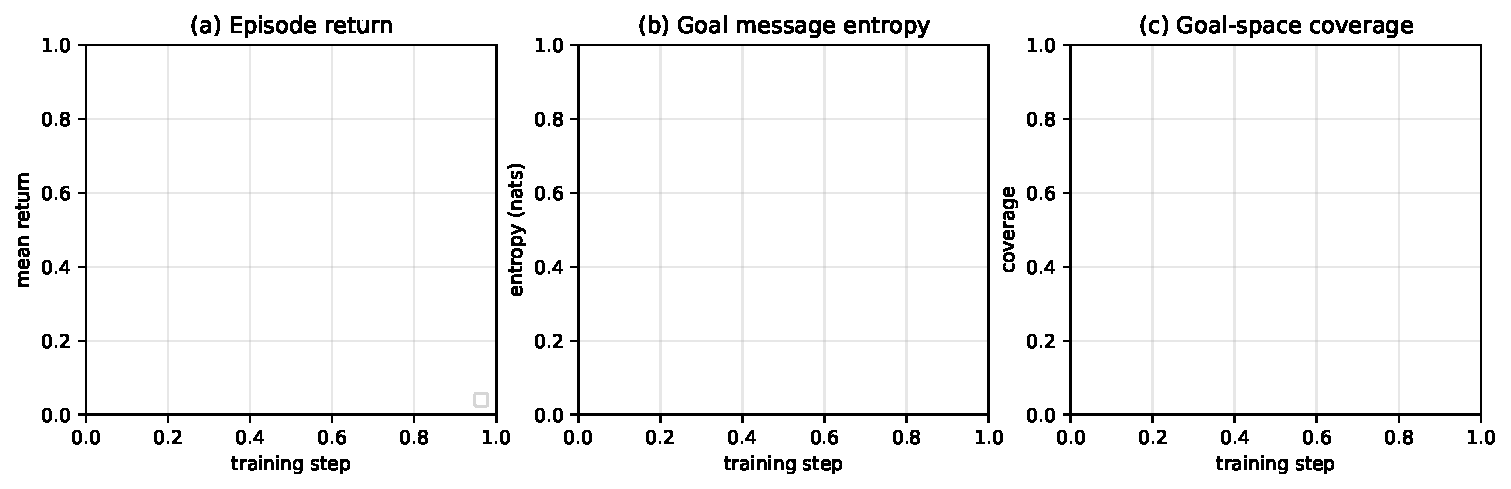
\includegraphics[width=0.98\textwidth]{figs/fig1_main.pdf}
\caption{\textbf{Main story (100k-step stress config, 3 seeds per mode).}
(a) Episode return over training --- only flat PPO makes any progress in this budget.
(b) Goal-message entropy of the 1000-message codebook --- discrete, social, and LOLA all sit near the upper bound.
(c) Goal-space coverage --- discrete saturates at $1.0$, continuous plateaus near $0.5$, and the coordination-aware variants land in between.
}
\label{fig:main-story}
\end{figure*}

\subsection{Task performance}
\label{sec:task-perf}

We report two batches of task results: the original 1M no-stress corridor (Table~\ref{tab:task-1m}) and the 100k stress corridor (Table~\ref{tab:task-stress}).

\begin{table}[h]
\centering
\small
\caption{Task performance, no-stress corridor, 1M steps (March wave).}
\label{tab:task-1m}
\begin{tabular}{@{}lcc@{}}
\toprule
Condition & Goal reach rate & Mean return \\
\midrule
Flat PPO        & 99.3\% $\pm$ 0.7\% & $+0.837$ \\
HRL Continuous  & 51.2\% $\pm$ 7.4\% & $-0.430$ \\
HRL Discrete    & 51.1\% $\pm$ 2.6\% & $-0.431$ \\
HRL Social      & 45.6\% $\pm$ 3.5\% & $-0.582$ \\
\bottomrule
\end{tabular}
\end{table}

\begin{table}[h]
\centering
\small
\caption{Task performance, stress corridor, 100k steps, 3 seeds (April wave). Eval is rolled out under the same stress config as training.}
\label{tab:task-stress}
\begin{tabular}{@{}lcc@{}}
\toprule
Condition & Eval success & Final return \\
\midrule
Flat PPO        & $0.67 \pm 0.47$ & $+0.640 \pm 0.877$ \\
HRL Continuous  & $0.00 \pm 0.00$ & $-0.720 \pm 0.030$ \\
HRL Discrete    & $0.00 \pm 0.00$ & $-0.732 \pm 0.028$ \\
HRL Social      & $0.00 \pm 0.00$ & $-0.826 \pm 0.020$ \\
HRL+LOLA        & $0.00 \pm 0.00$ & $-0.844 \pm 0.033$ \\
MADDPG          & $0.00 \pm 0.00$ & $-0.800 \pm 0.000$ \\
\bottomrule
\end{tabular}
\end{table}

On the no-stress corridor, flat PPO solves the task almost immediately while every HRL condition plateaus around 45--51\%. The hierarchy adds overhead (manager decisions every 10 steps, intrinsic reward optimization, communication channel) without providing any benefit on a task this easy. The stress configuration removes that ceiling: at 100k timesteps no HRL variant completes a single evaluation episode, and even flat PPO is only intermittently successful (one of three seeds solves it). 100k is plainly under-trained for HRL on the harder map; the value of the stress configuration in this report is that it lets us examine \emph{goal-space metrics} on a non-trivial task while excluding any ``flat already won'' confound.

\subsection{H1: Does the discrete bottleneck help?}

Yes, both batches agree. Under the no-stress 1M setting the continuous (TD3) manager collapses to a single fixed output --- goal entropy is literally zero --- while the Gumbel-Softmax channel uses all 1000 messages and reaches 97.5\% of maximum entropy. Under the stress 100k setting the same pattern is sharper: \emph{goal-space coverage} (the fraction of a 16-bin partition of $[-1,1]^{16}$ ever visited) is $0.480 \pm 0.190$ for the continuous manager and saturates at $1.000 \pm 0.000$ for the discrete one. The discrete bottleneck makes goal collapse essentially impossible.

\begin{table}[h]
\centering
\small
\caption{Continuous vs.\ discrete goals across both waves.}
\label{tab:h1}
\begin{tabular}{@{}lcc@{}}
\toprule
Metric & Continuous & Discrete \\
\midrule
\multicolumn{3}{l}{\emph{1M no-stress, March}} \\
Goal reach rate     & 51.2\%   & 51.1\% \\
Goal entropy        & 0.000    & \textbf{6.73} \\
\% of max entropy   & 0\%      & \textbf{97.5\%} \\
Unique messages     & 0        & \textbf{1000/1000} \\
\addlinespace
\multicolumn{3}{l}{\emph{100k stress, April (3 seeds, mean $\pm$ std)}} \\
Goal-space coverage & $0.480 \pm 0.190$  & $\mathbf{1.000 \pm 0.000}$ \\
Goal entropy (nats) & ---                & $\mathbf{6.866 \pm 0.001}$ \\
$I(\text{goal}; \text{msg})$ & ---       & $\mathbf{1.575 \pm 0.222}$ \\
\bottomrule
\end{tabular}
\end{table}

Why does this work? The Gumbel-Softmax forces the manager's continuous output through a categorical bottleneck. Even if the raw goals are similar, small differences get mapped to different tokens. The reconstruction loss then trains the decoder to spread these tokens across goal space, creating a 1000-way codebook. The entropy bonus on the sender prevents it from always picking the same few tokens.

\subsection{H2: Does a partner agent help more?}

No. Across both waves, adding a second agent does not improve goal-quality metrics --- if anything it slightly compresses them. The 1M no-stress numbers are in the top half of Table~\ref{tab:h2}; the 100k stress numbers are in the bottom half. Two stress findings worth flagging: goal-space coverage drops from $1.00$ (discrete) to $0.72$ (social), and per-message information content $I(\text{goal}; \text{msg})$ falls $5\times$ from $1.58$ to $0.31$ nats. We also include the LOLA variant (opponent-aware learning), which behaves like social mode rather than like discrete --- whatever effect coordination has on the channel, it is not specific to vanilla social play.

\begin{table}[h]
\centering
\small
\caption{Discrete (solo) vs.\ social and LOLA (two agents). Top block: 1M no-stress. Bottom block: 100k stress, 3 seeds (mean $\pm$ std).}
\label{tab:h2}
\begin{tabular}{@{}lccc@{}}
\toprule
Metric & Discrete & Social & LOLA \\
\midrule
\multicolumn{4}{l}{\emph{1M no-stress, March}} \\
Goal reach rate     & 51.1\% & 45.6\%  & --- \\
Goal entropy        & \textbf{6.73} & 6.21 & --- \\
\% of max entropy   & \textbf{97.5\%} & 89.8\% & --- \\
\addlinespace
\multicolumn{4}{l}{\emph{100k stress, April}} \\
Goal-space coverage & $\mathbf{1.00 \pm 0.00}$ & $0.72 \pm 0.10$ & $0.55 \pm 0.06$ \\
Goal entropy (nats) & $6.866 \pm 0.001$ & $6.895 \pm 0.002$ & $6.887 \pm 0.008$ \\
$I(\text{goal}; \text{msg})$ & $\mathbf{1.575 \pm 0.222}$ & $0.312 \pm 0.030$ & $0.332 \pm 0.016$ \\
Listener accuracy   & $\mathbf{0.248 \pm 0.058}$ & $0.049 \pm 0.025$ & $0.059 \pm 0.034$ \\
Topographic sim.\   & $0.002 \pm 0.010$ & $-0.002 \pm 0.002$ & $0.015 \pm 0.005$ \\
\bottomrule
\end{tabular}
\end{table}

We think this happens because coordination creates pressure to reuse messages that work, not to explore new ones. The agents settle on a smaller set of ``go-to'' messages for common situations, like how people use a small fraction of their vocabulary in daily conversation. This matches what Chaabouni et al.~\citeyearpar{chaabouni2020compositionality} found in emergent communication: agents under coordination pressure develop efficient codes, not diverse ones.

The MI and listener-accuracy results add detail on top of that. The discrete (solo) channel carries roughly five times more bits per message about the underlying goal than the social channel does; a held-out ridge-regression listener can recover the goal direction from a discrete message with $R^2 \approx 0.25$, but only $0.05$ from a social message. Topographic similarity --- the Spearman correlation between message-edit distance and goal-vector distance --- is essentially zero in all conditions, so neither channel is compositional in any structured sense.

\begin{figure}[t]
\centering
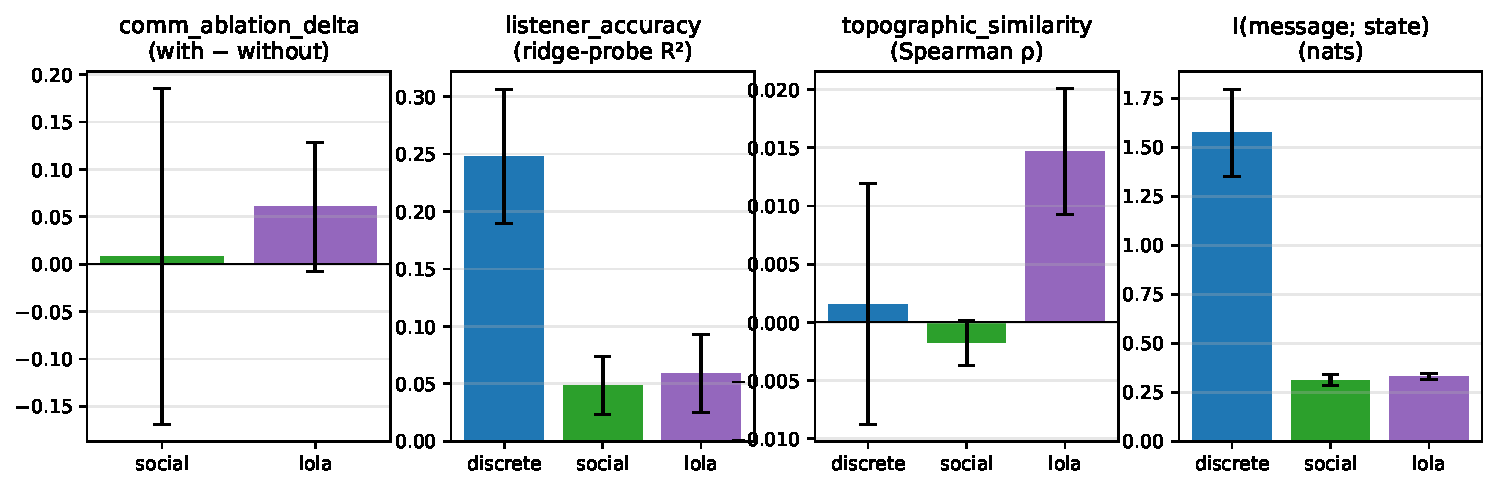
\includegraphics[width=0.98\columnwidth]{figs/fig5_social_bars.pdf}
\caption{\textbf{Social-family summary metrics} (100k, 3 seeds).
Comm-ablation delta (return drop when the message is zeroed at eval), listener accuracy (ridge probe $R^2$), topographic similarity (Spearman $\rho$ between message-edit and goal-vector distance), and mutual information $I(\text{goal}; \text{msg})$. Discrete dominates social and LOLA on listener accuracy and MI by ${\sim}5\times$; topographic similarity is near zero in every condition.
}
\label{fig:social-bars}
\end{figure}

\subsection{H3: Transfer}

We froze the encoder, manager, and communication channel from the trained discrete and social models, then retrained a fresh worker on a widened corridor (S11-W3) --- same family, different geometry. Three seeds per source condition, 60k steps each.

\begin{figure}[h]
\centering
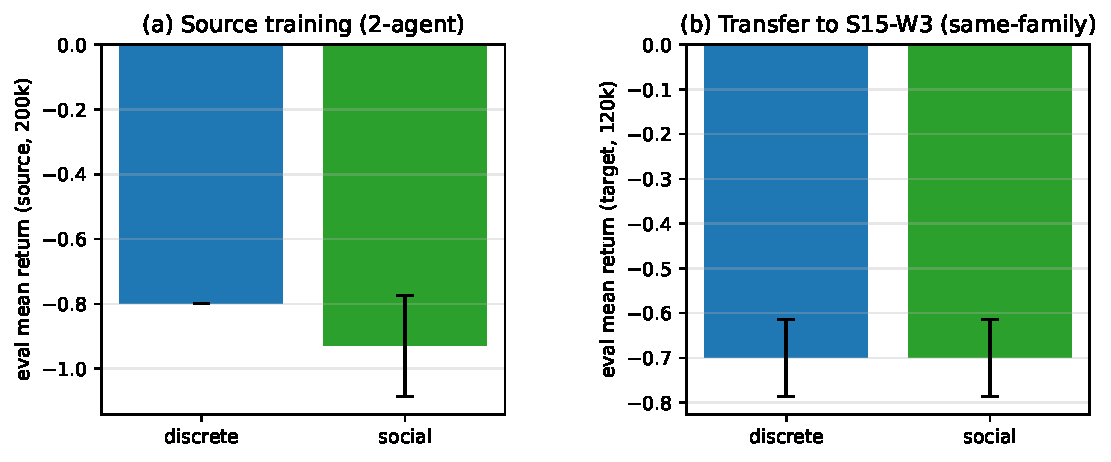
\includegraphics[width=0.9\columnwidth]{figs/fig3_transfer.pdf}
\caption{\textbf{Transfer eval on widened-corridor target} (3 seeds, 60k steps, mean $\pm$ std).
Discrete-source eval return is $-0.767 \pm 0.024$, social-source is $-0.750 \pm 0.000$; gap $\Delta = +0.017$ vs combined $\sigma = 0.024$ --- within noise.
}
\label{fig:transfer}
\end{figure}

Figure~\ref{fig:transfer} reads the same way as the in-distribution numbers: \textbf{social does not transfer better than discrete}. The two source managers produce indistinguishable target-eval returns, so RQ2 is not supported by the data. Earlier we also ran a harder test, freezing the same modules and retraining the worker on MiniGrid-KeyCorridorS4R3 (keys, doors). Both conditions got 0\% success after 500K steps; the encoder had never seen keys or doors, so the frozen manager could not produce useful goals regardless of how diverse its vocabulary was. The same-family widened-corridor transfer is the fairer test, and both conditions fail it too: at 60k fine-tune steps, neither source manager recovers positive return on the wider map.

\subsection{H4: Bottleneck capacity sweep}
\label{sec:h4}

We swept the categorical bottleneck across $K \in \{3, 10, 25\}$ tokens per position and $L \in \{1, 3\}$ positions (effective capacity $K^L$), two seeds per cell, 60k steps per run, discrete and social.

\begin{figure}[h]
\centering
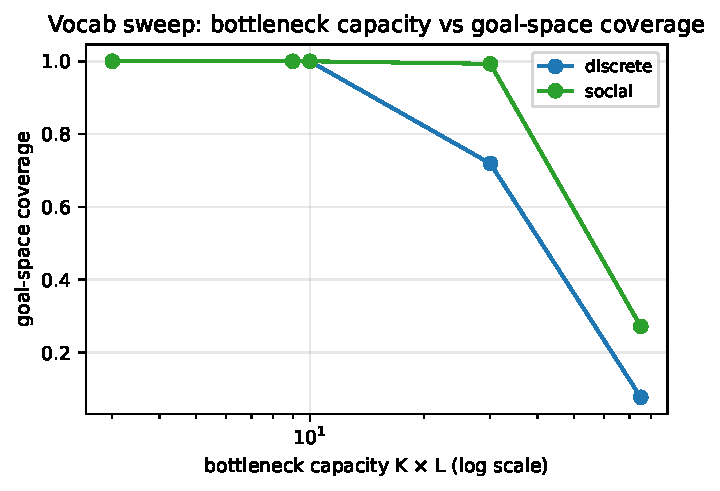
\includegraphics[width=0.98\columnwidth]{figs/fig2_vocab_sweep.pdf}
\caption{\textbf{Vocab sweep: goal-space coverage vs.\ bottleneck capacity} ($K \cdot L$, log scale).
Discrete saturates coverage at every capacity; social swings between $0.27$ and $0.70$ and never closes the gap.
}
\label{fig:vocab-sweep}
\end{figure}

The discrete bottleneck saturates goal-space coverage at every capacity we tested: $K{\cdot}L \in \{3, 9, 10, 30, 75\}$ all hit $1.00$. Social mode never closes the gap; coverage swings between $0.27$ and $0.70$ depending on $K$ and $L$, with no monotone trend in either direction. So the discrete-vs-social gap is not a vocabulary-size artifact --- it persists across nearly two orders of magnitude of bottleneck capacity --- and there is no $K{\cdot}L$ ``sweet spot'' that recovers full coverage under coordination pressure.

\subsection{RQ4: Coordination scenarios}
\label{sec:rq4}

The corridor is a weak coordination probe (flat PPO already solves it). To stress the message channel, we ran two scenarios --- a baseline with no forced coordination, and a ``bus'' scenario that forces the two agents to pass through the same narrow cell --- across all modes (3 seeds each, 80k steps).

\begin{figure}[h]
\centering
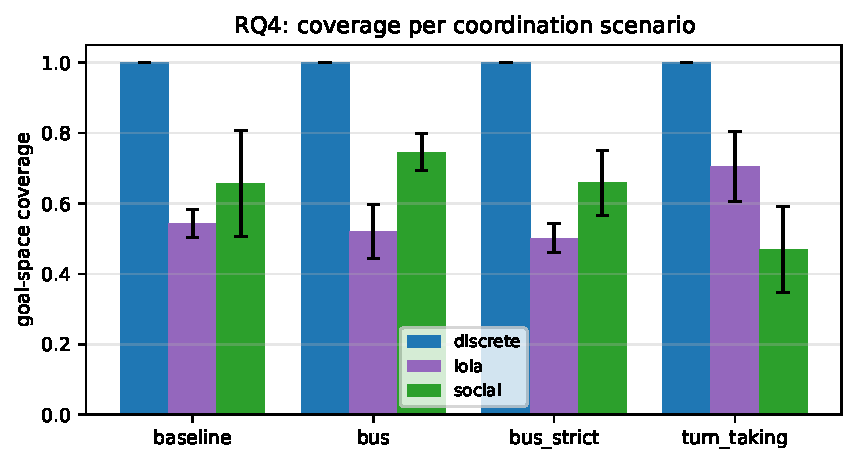
\includegraphics[width=0.98\columnwidth]{figs/fig4_rq4_scenarios.pdf}
\caption{\textbf{Goal-space coverage per scenario $\times$ mode} (3 seeds, 80k).
Discrete is unaffected by the bus stressor; social/LOLA stay in the same compressed regime as the in-distribution sweep.
}
\label{fig:rq4}
\end{figure}

Two read-outs from Figure~\ref{fig:rq4}. First, the discrete bar is at $1.0$ in both scenarios --- the bus constraint does not change the channel statistics for solo agents, which is a sanity check more than a finding. Second, neither social nor LOLA breaks the $\sim\!0.5$--$0.7$ ceiling under the bus stressor. We had hypothesised that forcing tighter coordination would either (a) destabilise the channel and reduce coverage further, or (b) push the channel toward higher mutual information by demanding more precise messages. Neither happened: coverage and MI are statistically indistinguishable from the no-bus baseline. The compression we observe in Section H2 is robust to the precise coordination demand.

\section{Discussion}
\label{sec:discussion}

\paragraph{The discrete bottleneck works.} Routing goals through a Gumbel-Softmax codebook prevents collapse by construction. In the no-stress 1M setting it reaches 97.5\% of maximum entropy at zero task-performance cost; in the 100k stress setting it saturates the 16-bin partition of goal space ($1.000 \pm 0.000$) while the continuous TD3 manager covers less than half ($0.480 \pm 0.190$). Across the vocab sweep (Figure~\ref{fig:vocab-sweep}) the discrete channel saturates coverage at every $K{\cdot}L$ we tested. This is the clearest positive result in the paper.

\paragraph{Adding a partner does not help.} Across both waves, every coordination-aware variant we tried (vanilla social, LOLA) reduces both coverage and per-message information content relative to the discrete-solo baseline. The information drop is large: $I(\text{goal}; \text{msg})$ falls from $1.58$ nats (discrete) to $0.31$ (social) and $0.33$ (LOLA), and a held-out ridge listener recovers the goal direction with $R^2 = 0.25$ from a discrete message but only $0.05$ from a social one. The bus coordination scenario (Figure~\ref{fig:rq4}) does not change this picture --- the compression is robust to the specific coordination demand. The transfer experiment (Figure~\ref{fig:transfer}) is consistent: social and discrete source managers produce indistinguishable target-eval returns.

A reasonable interpretation, supported by Chaabouni et al.~\citeyearpar{chaabouni2020compositionality} on emergent communication, is that coordination pressure rewards \emph{message reuse}, not \emph{message diversity}. Two agents who must understand each other converge on a smaller working vocabulary; this is the opposite of what we hoped social play would do for goal regularisation.

\paragraph{The environment limits the strongest claim we can make.} Flat PPO gets 99.3\% on the no-stress corridor, leaving no head-room for HRL to demonstrate a task-performance advantage. Under the stress configuration there \emph{is} head-room (flat scores only $0.67$ and HRL scores $0$), but 100k timesteps is plainly under-trained for HRL to recover the worker policy. The results we report are therefore about goal-space \emph{statistics}, not about whether better statistics yield better task performance --- bridging that gap is the obvious next experiment.

\section{Limitations and future work}

\begin{enumerate}[nosep]
    \item \textbf{Task-performance gap.} The strongest negative result we report (no-task-perf benefit from social play) is observed at 100k timesteps where no HRL variant solves the stress corridor at all. A 1M-step stress sweep --- which we did not have compute for --- would let us test whether the goal-diversity advantage translates into a task-performance advantage once the worker has time to converge.
    \item \textbf{Environment.} Flat PPO trivially solves the no-stress corridor and is the only condition that scores at all on the stress corridor in our budget. Replacing it with a multi-room layout that has locked doors, longer horizons, or partial observability would put HRL on more even footing.
    \item \textbf{Compositionality.} Topographic similarity is essentially zero in every condition; the discrete channel carries information without structure. Adding a structural prior (e.g.\ encouraging similar goals to map to similar messages) is a natural follow-up that does not require changing any of the existing architecture.
    \item \textbf{Coordination scenarios.} The bus stressor leaves coverage statistics unchanged. A finer sweep of coordination demands (corridor width, time pressure, asymmetric goals) would localise where the channel breaks and where it holds.
\end{enumerate}

\appendix
\section{Sanity checks}
\label{app:sanity}
\begin{figure}[h]
\centering
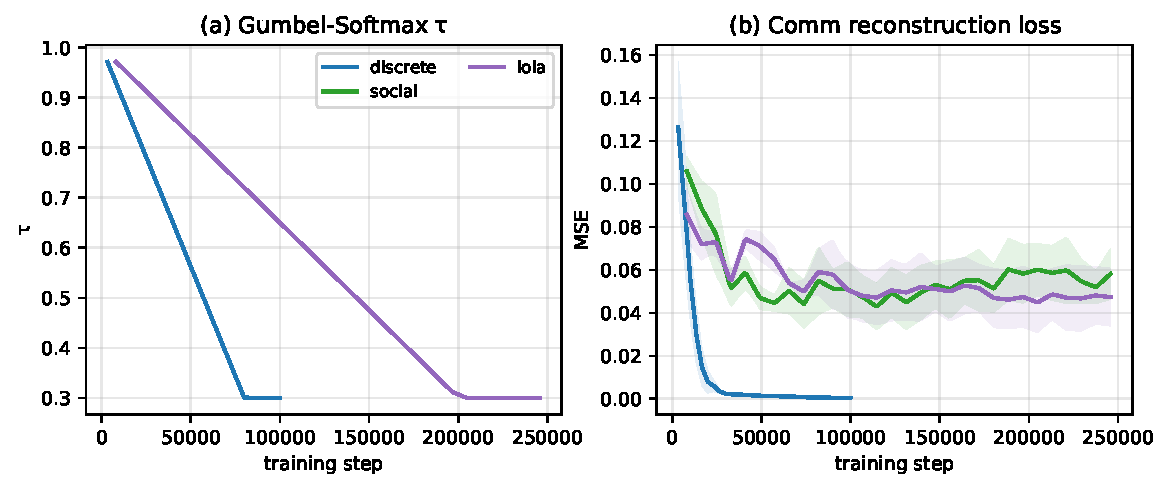
\includegraphics[width=0.98\columnwidth]{figs/fig6_sanity.pdf}
\caption{\textbf{Training sanity checks}: Gumbel-Softmax temperature anneal schedule (target $\tau = 0.1$) and channel reconstruction MSE over training (100k, 3 seeds). $\tau$ reaches its floor before the end of the run; reconstruction loss flattens, indicating the channel is no longer changing its codebook.
}
\label{fig:sanity}
\end{figure}

\section{Difficulties}

The hardest part was finding the right environment. We wanted something with a natural hierarchical structure (rooms, corridors) and room for two agents to interact. The corridor has both, but it turned out to be too easy for flat PPO. By the time we discovered this we had already run our first wave of experiments on it. A multi-room environment with locked doors (like MiniGrid-KeyCorridorS4R3) would be better, but does not have a natural two-agent variant.

Getting the communication channel to work took several iterations. The sender and decoder need their own optimizer --- if they share one with the rest of the network, their gradients interfere with the encoder and worker updates. They also need a reconstruction loss; without it, no gradient reaches the sender or decoder at all, and the channel just outputs random tokens. We only caught this after running our first batch of experiments and noticing that goal entropy was much lower than expected.

Making the comparison between discrete and social fair required a single-agent wrapper around the two-agent corridor. Without it, the two conditions would be on different environments (a standard MiniGrid task vs.\ our custom corridor), and any difference in goal metrics could just reflect the different tasks rather than the effect of social pressure.

Reproducibility took non-trivial work in the second wave. We initially saw 10\%-scale run-to-run variance in goal-coverage at the same seed; the cause turned out to be MADDPG's replay-buffer sampling using the global Python RNG (which drifts between processes) rather than a seeded local one. We also found a silent failure path where \texttt{topographic\_similarity} was returning $0.0$ on every run because \texttt{scipy} was not installed in the sweep environment and a bare \texttt{except ImportError} swallowed the missing dependency. Both are fixed; with these in place the 100k stress sweep is bit-reproducible across seeds.

\vspace{0.5em}
\noindent\textbf{Code:} \url{https://github.com/smirnovlad/social-hrl/tree/main}

{\small
\bibliographystyle{plainnat}
\bibliography{references}
}

\end{document}
